\documentclass[10pt]{article}
\usepackage[letterpaper,landscape,margin=0.65in]{geometry}
\usepackage{graphicx}
\usepackage{booktabs}
\usepackage[T1]{fontenc}
\usepackage{hyperref}
\hypersetup{pdftitle={BINSTD source provenance and policy attribution audit}}
\setlength{\parindent}{0pt}
\setlength{\parskip}{0.5em}
\title{BINSTD source provenance and policy attribution audit}
\author{Validation audit, 22 October 2026}
\date{}
\begin{document}
\maketitle
\vspace{-2em}

\textbf{Question.} Does frozen evidence record \texttt{EV-BINSTD-030b4e}
attribute its five internal citations and infrastructure policy accurately?
The record says Stage 1 could not measure the charged-cost band because the
shared XOR-SAT pin was absent. This audit changes no experiment or verdict.

\textbf{Source reading.} The hypothesis, frozen n=17 experiment, approval
decision, source proposal's wider heuristic, and \texttt{AGENTS.md} were read.
The approved experiment tests $n=17$, $\ell\in\{3,4\}$ with at least 40
matched targets and a shared solver pin. The proposal's heuristic also names
$n=19,23$, but neither was admitted in this Stage-1 test. The approval is not
scientific support. No charged-cost comparison occurred after the pin was
found absent.

\textbf{Correction.} The frozen evidence cited \texttt{AGENTS.md} core rule 3
for treating an infrastructure failure as non-mathematical evidence. Rule 3
concerns experimental design. Core rule 5 says timeout, crash or
implementation failure is not mathematical evidence. A hash-bound additive
replacement corrects three rule references and adds five source-reading
notes. The frozen record is unchanged. A focused structured-diff checker
confirms no other field changed.

\textbf{Validation.} The original SHA-256 begins \texttt{a65bd7986a54}; the
replacement begins \texttt{159c0d02cac5}. The companion receipt records
structured equality and the complete-tree validator's exact delta. On
current base \texttt{13eb21767865}, unsuppressed errors fell from 141 in
39 paths to 136 in 38 paths: exactly five citation errors removed, none added.
Both runs still exit 1, so the all-corpus gate remains red.

\textbf{Boundary.} Stage 1 remains an implementation impediment, not a
measurement or falsification of the heuristic. No run, timing, performance
curve, attack-cost bound, or scientific decision changed.

\newpage
\begin{center}
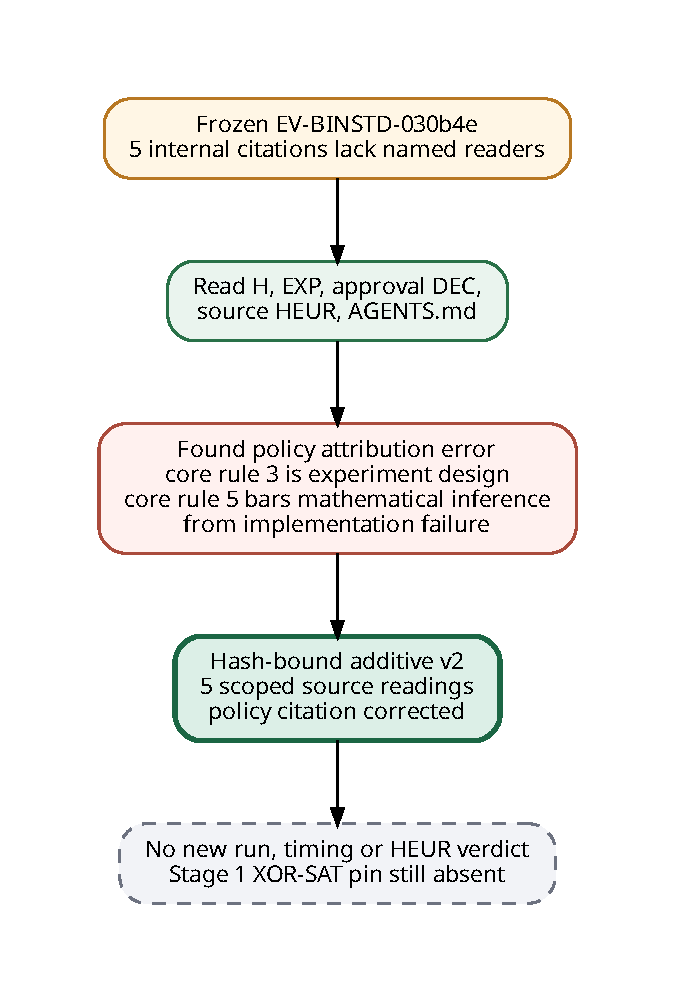
\includegraphics[width=\textwidth,height=0.82\textheight,keepaspectratio]{audit-figure.pdf}
\end{center}
\end{document}
